% Hur är gloria designat i ett macro-perspektiv

\section{Systemet}
Systemet GLORIA består av fyra enheter. En PCenhet som styr låter användaren styra systemet och läsa debugdata, en styrenhet som sköter drivningen av robotarm och motorer, en sensorenhet som kontinuerligt läser sensordata och en huvudenhet som tar emot kommandon från PCenheten och avgör vad roboten skall göra. Hur dessa enheter hänger ihop illustreras i figur \ref{system-oversikt}.

\begin{figure}[h!]
	\centering
	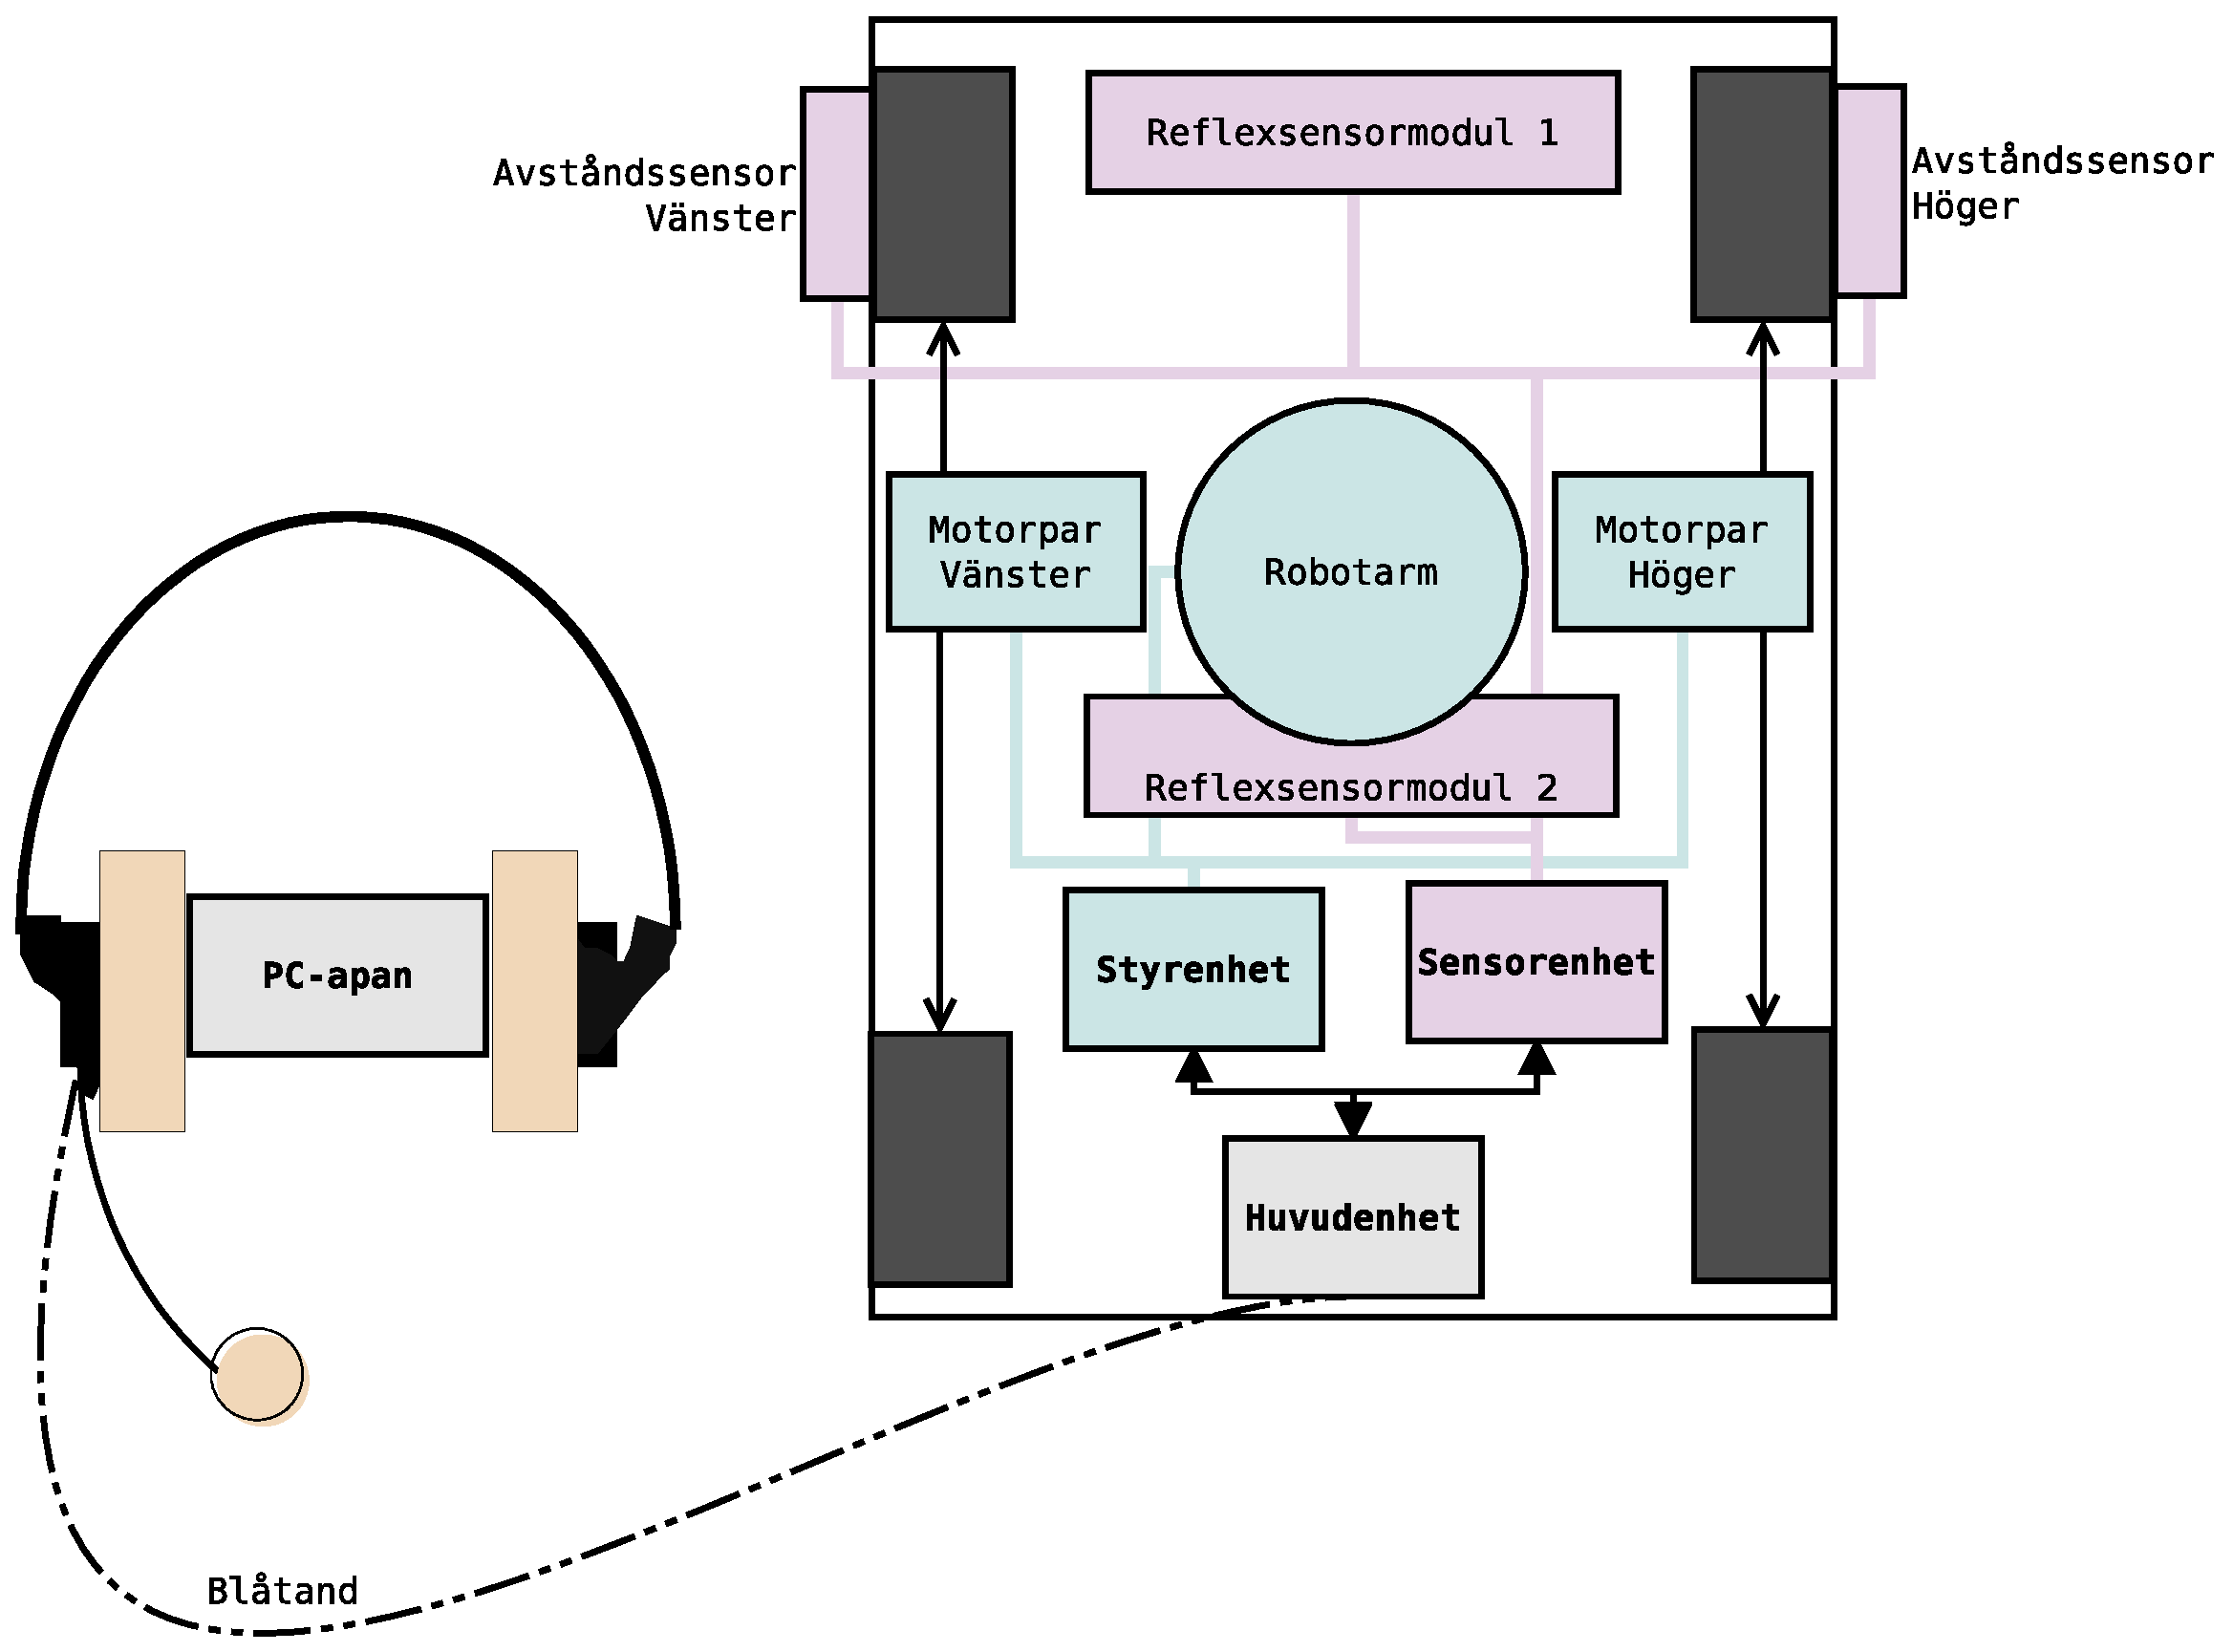
\includegraphics[scale=0.4]{grafik/system-oversikt}
	\caption{Översikt av systemet} \label{system-oversikt}
\end{figure}

PCenheten innefattar ett grafiskt gränssnitt där man kan se debugmeddelanden, sensordata, motorhastigheter och armens position. I det grafiska gränssnittet finns reglage för att bestämma om systemet är i sitt manuella eller autonoma läge. När systemet är i sitt manuella läge styrs det med två joysticks via det grafiska gränssnittet.

Huvudenheten innehåller robotens intelligens, den tar beslut om vad som ska göras beroende på om roboten är i sitt manuella eller autonoma läge. I det autonoma läget är det i huvudenheten all styrlogik finns som säger vart roboten är och vad den ska göra. Det är även där regleringen ligger som ser till att roboten följer banan.

Sensorenheten förser huvudenheten med sensordata.

Styrenheten tar instruktioner från huvudenheten och ser till att motorer och servon utför dessa.
